\documentclass[15pt]{article}
\usepackage[utf8]{inputenc}
\usepackage[main=french]{babel}
\usepackage{geometry}
\geometry{hmargin=2.5cm,vmargin=3cm}
\usepackage{graphicx}
\usepackage{amsfonts}
\usepackage{ulem}
\usepackage{amsmath}
\usepackage{esint}
\usepackage{calc}
\usepackage{array, multirow, makecell}
\usepackage{caption}
\usepackage{subcaption}
\usepackage{longtable}
\usepackage{multicol}
\usepackage{float}

\newcolumntype{R}[1]{>{\raggedleft\arraybackslash }b{#1}}
\newcolumntype{L}[1]{>{\raggedright\arraybackslash }b{#1}}
\newcolumntype{C}[1]{>{\centering\arraybackslash }b{#1}}

\title{\LARGE\textsc{{Génie Industriel}}}
\author{AlexCast}
\date{2019/2020}

\begin{document}

\begin{titlepage}
\begin{center}
    \vspace*{\stretch{1}}
$$   \begin{array}{cc}
        \mbox{\Huge\textsc{{Machine Learning}}}\\
        \mbox{Alexandre Castelnau}\\
        \mbox{Fall 2021}
    \end{array}$$
    \vspace*{\stretch{1}}
\end{center}
\begin{figure}[b]
    \centering
    
\includegraphics[width=10cm]{GT-logo.jpg}
\end{figure}
\end{titlepage}
\newpage

\tableofcontents
\newpage

\begin{multicols}{2}

\section{Introduction - Description of the datasets}

I decided to take once again the two datasets I have previously taken during the first assignment: the first one on hospital mortality, the second one on BMW cars. All the datasets have been retrieved in CSV format and are put in a Pandas DataFrame. Let's briefly summarize the characteristics of these datasets.

\subsection{Hospital mortalily}

\begin{figure}[H]
\centering
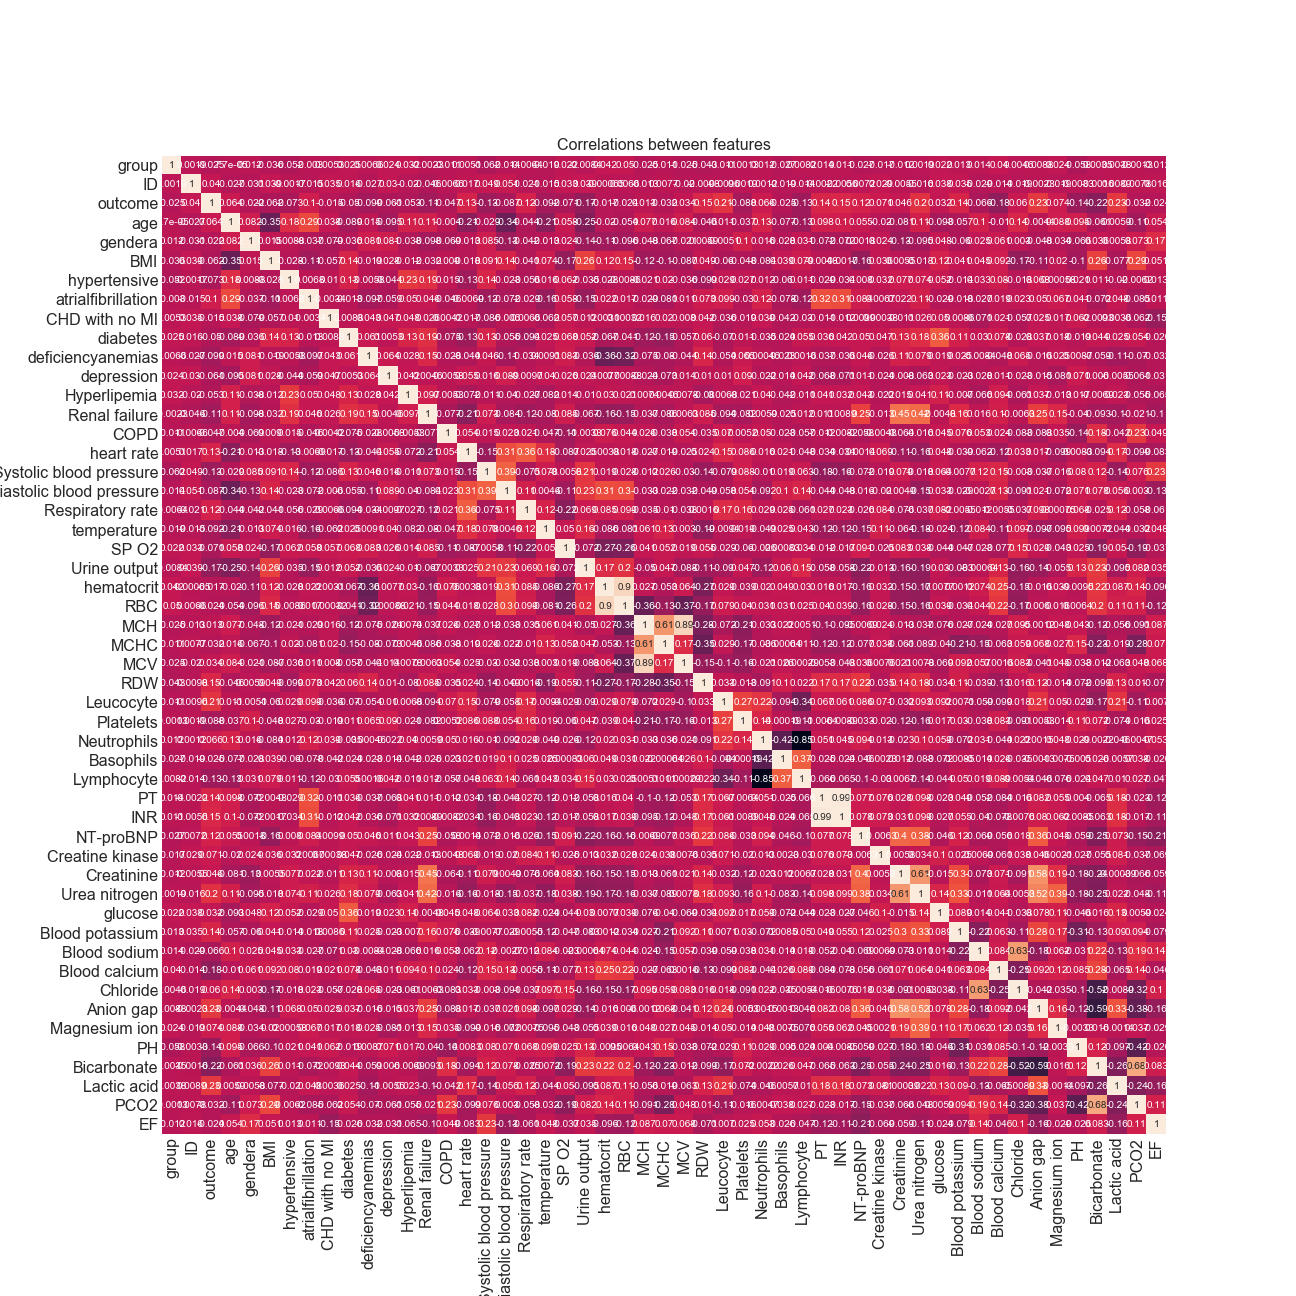
\includegraphics[width = \columnwidth]{corrFeatures.png}
\caption{Correlation between features}
\end{figure}

The hospital mortality dataset includes 1177 tuples. Each of these tuples compiles dozens (roughly 50) of attributes on each patient (age, gender, BMI, diabetes...). Later on, we will try to reduce the dimensionnality of this dataset. Among them, the binary attribute "outcome" represents the data that we will have to predict when we will try to use a neural network model. "Outcome" is 0 if the patient came out of the hospital alive and 1 if he died. It appears therefore that this first problem is a pure binary classification problem.

During the preprocessing phase, for each features if values were missing, I filled these values by the mediane of the feature. Also, I used a \textit{Standard Scaler}, to scale the dataset.

Moreover, it appears clearly that the problem is little bit hard because of the relative small size of the dataset, the fact that high predictive attributes (showing high value of correlation with the \textit{Outcome} attribute) don't exist here (unlike the following problem), and due to the unbalanced dataset (1018 people lived and 159 died). The figure above shows the correlation matrix (colors represent values: darker = lower values, lighter = higher values).

\begin{figure}[H]
\centering
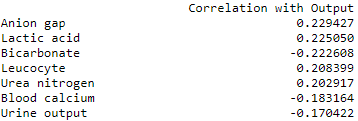
\includegraphics[width = \columnwidth]{Capture.png}
\caption{Features with greatest correlations}
\end{figure}

\subsection{BMW cars}

\begin{figure}[H]
\centering
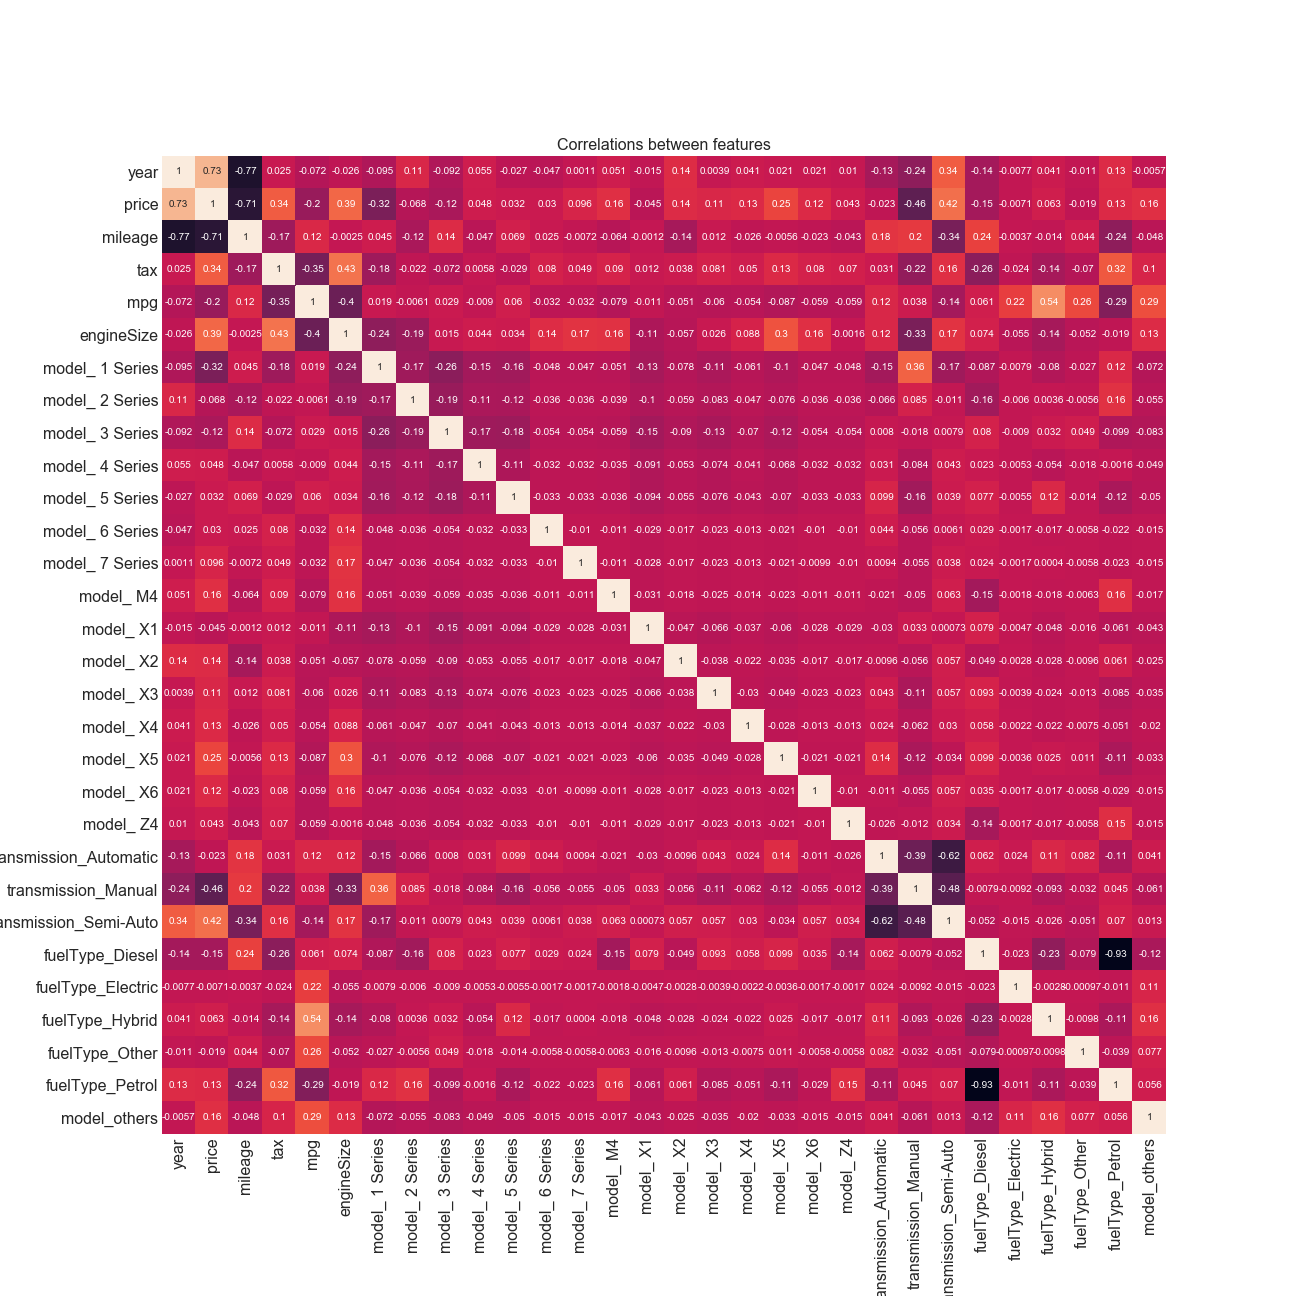
\includegraphics[width = \columnwidth]{corrFeaturesBMW.png}
\caption{Correlation between features}
\end{figure}

The BWM car dataset contains 10781 tuples. For each of the training points, we find the mileage, the model, the year of sale on the market, the engine size... The first purpose of all these attributes is to be able to predict the "Price" attribute which is the resale price of the vehicle in question. So, it's a regression problem. I turned it into a classification problem by using "boxes". For instance prices under 10000€, I labelled the tuple with the value 0, prices between 10000 and 15000€, the label 2...  We are now considering a multi-label classification problem (6 different labels).

During the preprocessing phase, I turned categorical features into numerical ones with \textit{One Hot Encoder}. I also used a \textit{Standard Scaler} over the previous numerical features.

We can observe that the correlation between price and some other attributes is very high, this might tend to facilitate the construction of predictive models. 

\begin{figure}[H]
\centering
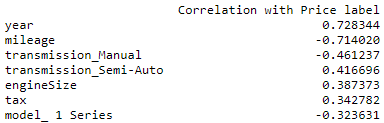
\includegraphics[width = \columnwidth]{Capture1.png}
\caption{Features with greatest correlations}
\end{figure}

\subsection{Brief statistical analysis of the dataset features}

Later, we will use several dimensionnality reduction algorithms. One of them is ICA and is well-known to be a solution or the cocktail party problem (in signal processing). To be able to use the ICA, one of the different assumptions is that the "sources" (here the different features) are zero-mean and have non-Gaussian distributions. We want non-Gaussian distributions because symmetries in Gaussian distributions can messed up the ICA search for independant directions.

We can easily tackle the first part of the assumption for any features by substracting the mean of the feature (the use of the \textit{Standard Scaler} allows us to have zero-mean features). But, for the second part is more independant of our will.

Hence, we can use our time navigating through datasets to see if the different features have non-Gaussian distributions. One of the thing we can observe to "measure non-Gaussianity" is the different moments of our data. Indeed, the moments of a distribution can defined it, so we can compare those to the one of a Gaussian. First and second moment (mean and variance) will not be useful (and the fact I use \textit{StandardScaler} set them to $\mu = 0$ and $\sigma^2=1$). So we can try to compute the third or fouth moments. The fourth moment, the Kurtosis:
$$ K = \mathbb{E}\left[ \left( \frac{X-\mu}{\sigma} \right)^4 \right] \text{ or } K_{norm} = \mathbb{E}\left[ \left( \frac{X-\mu}{\sigma} \right)^4 \right] - 3$$
can be compute easier, so let's look at it. 
For each feature, I was able to:
\begin{itemize}
\item Compute the Kurtosis value
\item Run an hypothesis test in which the null hypothesis is "Feature follows a normal distribution".
\end{itemize}

\begin{figure}[H]
\centering
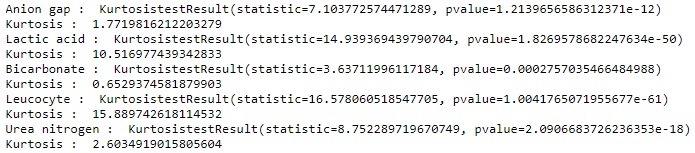
\includegraphics[width = \columnwidth]{Capture2.png}
\caption{Some results from the Hospital dataset}
\end{figure}

\begin{figure}[H]
\centering
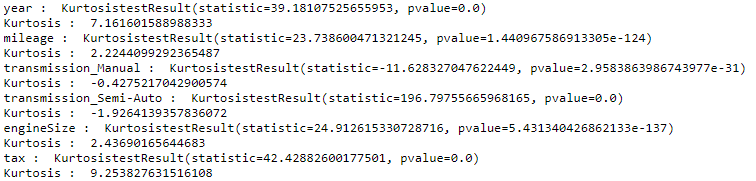
\includegraphics[width = \columnwidth]{Capture3.png}
\caption{Some results from the BMW dataset}
\end{figure}

In the results I plotted, there is the kurtosis, the Z-score and the p-value of the test. For each features, we can observe that the kurtosis is not equal  to 0 (the expected value for Gaussian distributions). Also, we observe large Z-scores and very small p-values that confirm us that we don't have Gaussian distribution. Indeed, the interpretation of a p-value can be "probability that the difference between what we see and what we expected for the null hypothesis is due to random chance". And if we set the confidence level at 95\% (and thus $\alpha=0.05$), the null hypothesis could be retained in the case where the Z-score is between plus or minus 2 (case of a two-sided test). Here, most of the tests return Z-scores that are not even close to these threshold values.

\section{Clustering algorithms}

First, in our exploration of the different algorithms, we will try to run the clustering algorithms (\textit{K-Means} and \textit{Expectation Maximization} on the BMW and hospital datasets.

\subsection{K-Means}

\subsubsection{The method}

When we try to use a clustering method, we must defined some hyperparameters. To see this more clearly, we can try clustering as an optimization problem defined as follows: considering N points in any space, find $k$ subspaces forming a partition that reflects the similarity of the points.
For \textit{KMeans}, we consider a distance function $d$ (or another function that can be tied with similarity) and $k$ centers ($c_{i<k}$). We define how the algorithm fit the data like that:
$$ F_k = \sum_{i=0}^{k-1} \sum_{x\in G_i} d(x, c_i) $$
So the output of the algorithm is the optimized centers $c_i$. But, we can see clearly that if $k_1>k_2$, $F_{k_1}>F_{k_2}$. Hence, choosing the hyperparameter $k$ is very important.

\begin{figure}[H]
\centering
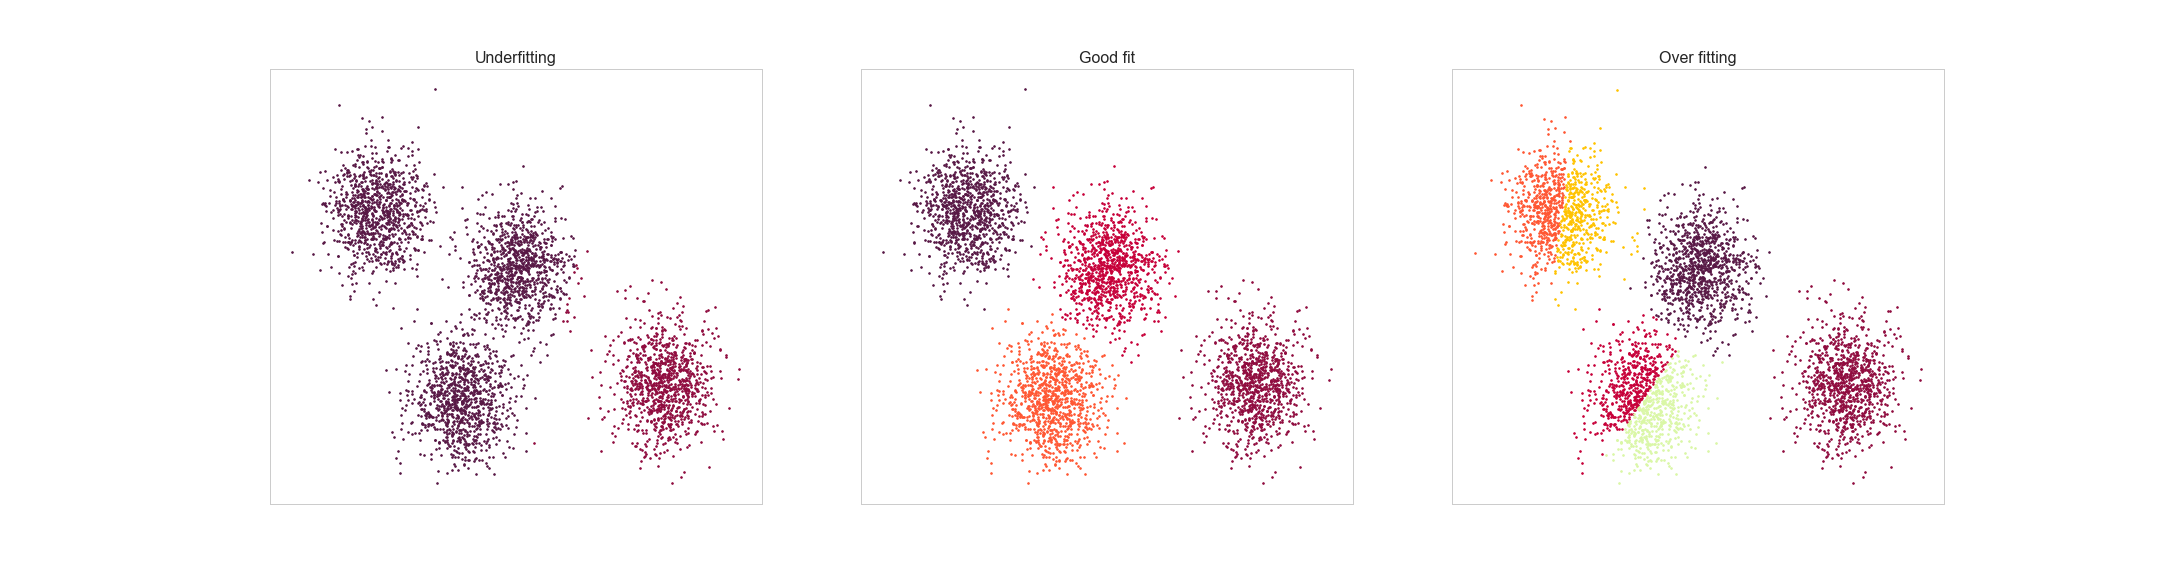
\includegraphics[width = \columnwidth]{blob.png}
\caption{Examples of clustering}
\end{figure}

Indeed, if we define a value that is too low, the clustering will not necessarily reflect how the data are articulated and this is also true for too high values. 
This is why we will try to use the elbow method to try to define the value of the hyperparameter that will give the most information. This corresponds to the moment when the precision of the output of the algorithm does not evolve at the same rate as at the beginning. It is simply a tradeoff between overfitting and underfitting.

\begin{figure}[H]
\centering
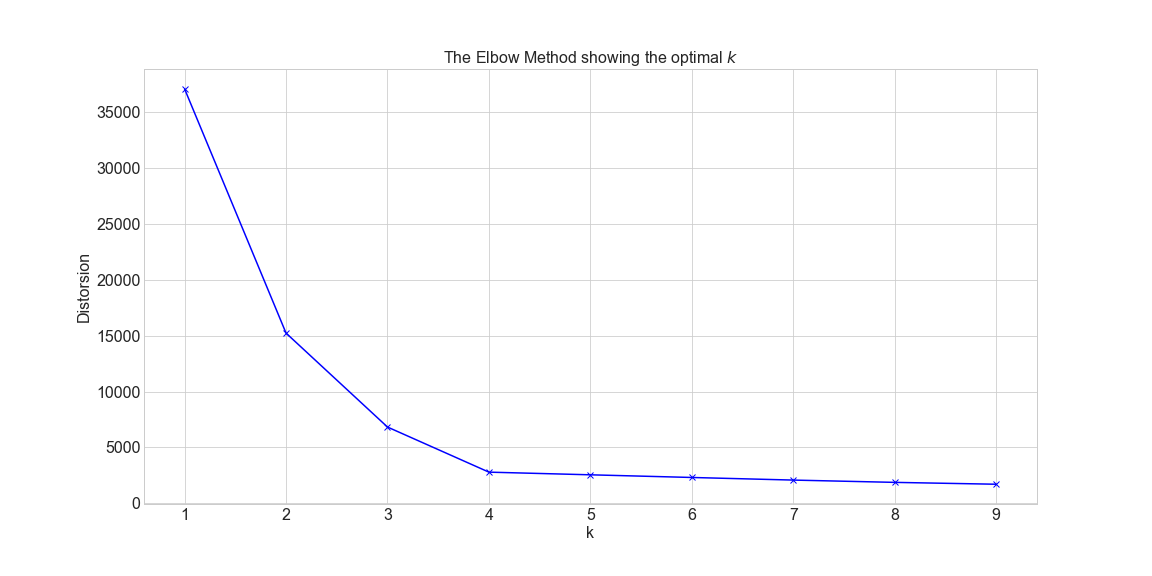
\includegraphics[width = \columnwidth]{elbowblob.png}
\caption{Elbow method over the example}
\end{figure}

In the little example I plotted, we can see four clear distinct groups, the elbow method allows us to detect the number of clusters. Meanwhile, it is a very simple example, our datasets are way more complex and detecting cluster will not be easy like that.

\subsubsection{KMeans on the datasets}

We try to use the elbow method on the two datasets. But our data are way more messier than the previous example. It seems that finding a clear value of $k$ is almost impossible.

\begin{figure}[H]
\centering
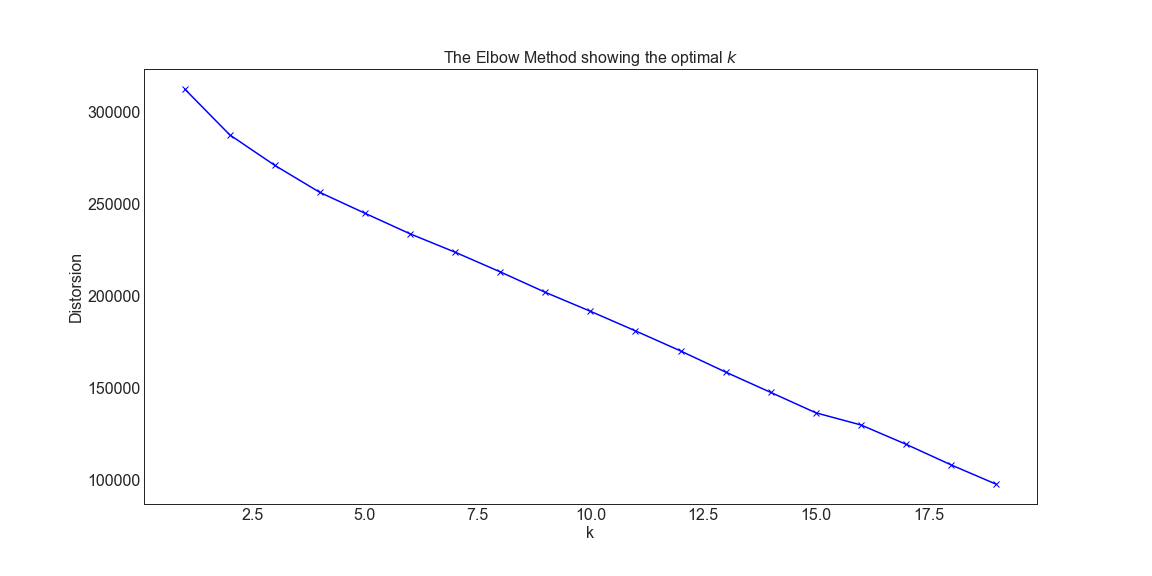
\includegraphics[width = \columnwidth]{elbowkm.png}
\caption{Elbow method (BWM initial data)}
\end{figure}

Since I was not able to define a clear value for the hyperparameter, I arbitrarily chose to take the number of labels existing for the supervised learning problem to see what the algorithm can bring us. I then projected these clusters against different features to observe them.

\begin{figure}[H]
\centering
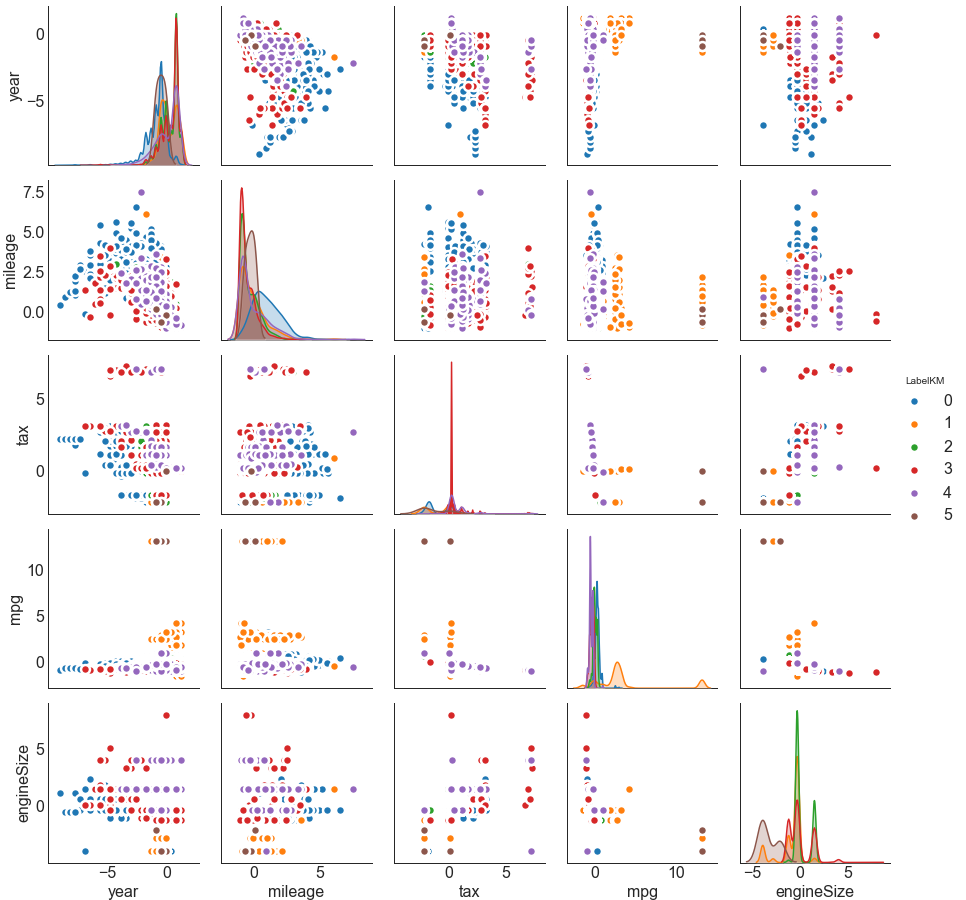
\includegraphics[width = \columnwidth]{pplotBMWkm.png}
\caption{Cluster projections (KM - BWM initial)}
\end{figure}

Nevertheless, the algorithm already seems to show some logical structures to find the price labels. For example, some of these clusters seem to gather the oldest and the most driven vehicles together (the most affordable in terms of price?), or the most powerful and the newest together (the most expensive?). We should try to see if what we think is verified when we compared it with labels.

So I took advantage of this operation to show the link between the clusters from KMeans and the price labels that exist in the supervised problem.

\begin{figure}[H]
\centering
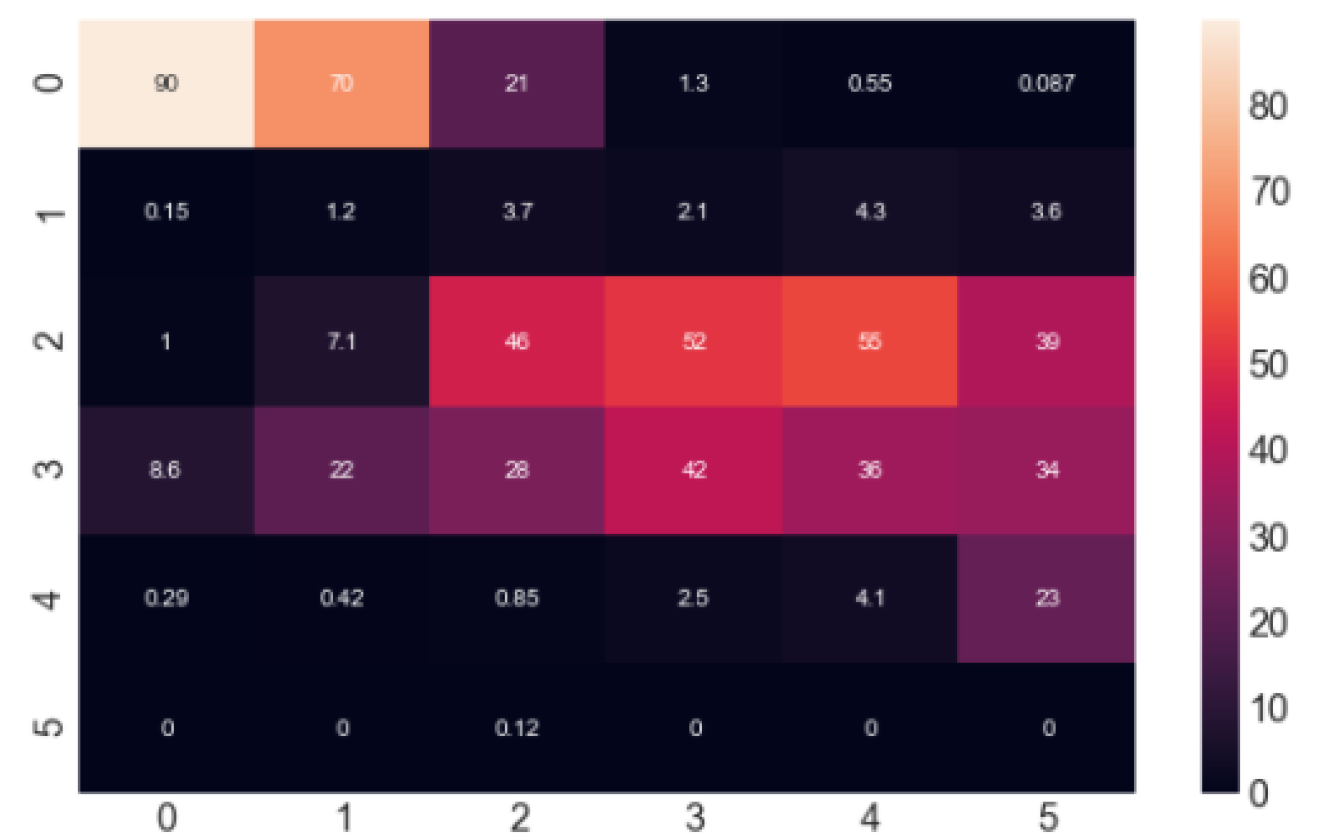
\includegraphics[width = \columnwidth]{grBMWkm.png}
\caption{Link between clusters and labels (HOS)}
\end{figure}

What this chart means? Rows are clusters and columns are labels. For instance, we can see that the cluster 0 contains 90\% of the data labelled by 0 and 70\% of the data labelled by 1 (cheap cars), and most expensive cars are mainly in the cluster 2 and 3.

\begin{figure}[H]
\centering
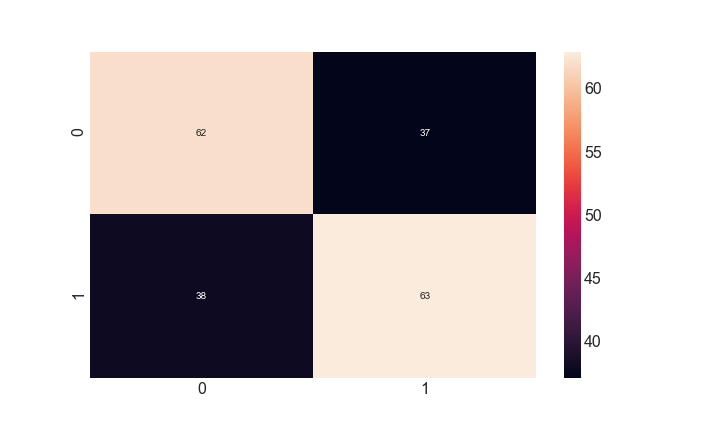
\includegraphics[width = \columnwidth]{grhoskm.png}
\caption{Link between clusters and labels (HOS)}
\end{figure}

All we said above is stil true when we use the mortality dataset. Inpretating the two cluster is little bit harder than with the BWF dataset. But we can clearly see that the two clusters don't respect the label but the proportion of dying patients is more inportant in the second cluster than the original dataset.



\subsection{Expectation Maximization}

\subsubsection{The method}

When we use the expectation Maximization, what we are doing is the following. We are trying to estimate the parameters $\theta$ of a Gaussian mixture from which we could extract the probabilities of a point and define the membership of a point to a cluster. To know how many gaussian variable I will consider for the mixture, I used the same parameter than in the KMeans.

For each data point, the algorithm returns an array giving us the probability that the point is in cluster $i$, so, to define what are the points in cluster $i$, we conserve the point where the maximum probability is for cluster $i$.

It is an iterative algorithm that allows us to "compute" Maximum Likelihood Estimates $\hat{\theta}$. To be exact it returns an approximation of the analytic solution (which may not be expressed). Each iteration, the algorithm tries to find random variables with simpler likelihood close to the distribution of our data and try to maximize the log-likelihook.

\subsubsection{EM applied to the dataset}

When we apply this clustering method on the BMW dataset, we can observe that the fact that we have values from categories or that take small distinct values affect the way EM works. Also, depending on the parameters that are found, we can find a cluster that predominates while the others would only deal with outliers. Here, this seems to be the case. The first cluster gathers most of the vehicles. This cluster therefore brings little or no information. 

However, in the context of medical data where the features take a much more diverse set of values (most of them take real values and are not limited to a restricted list), EM seems to be able to help us make sense of our data in the hope of building a future model allowing the prediction of the "outcome" feature. Indeed, it gives us two clusters: in the first one the proportion of dying is lower than in the intial dataset while in the second it is the opposite.

\begin{figure}[H]
\centering
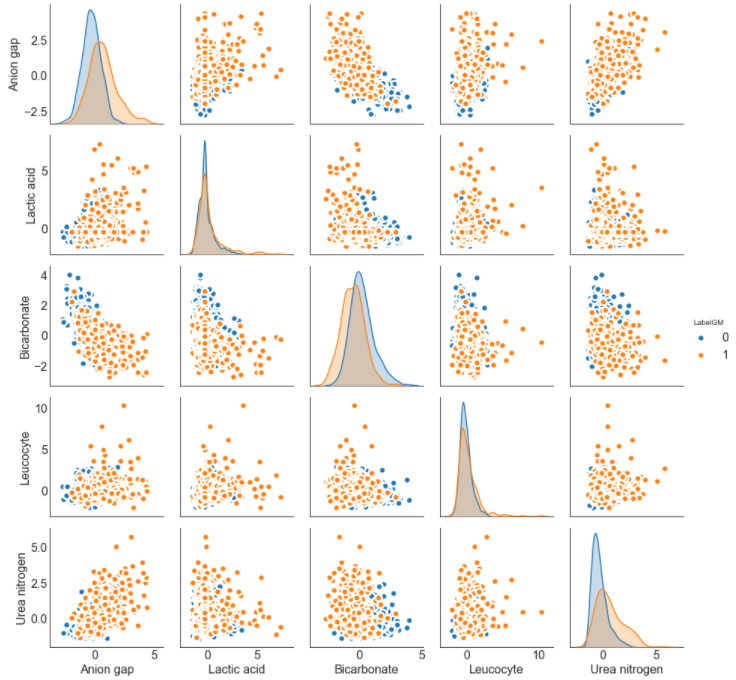
\includegraphics[width = \columnwidth]{pplothosgaus.png}
\caption{Cluster projections (EM - initial HOS)}
\end{figure}

\begin{figure}[H]
\centering
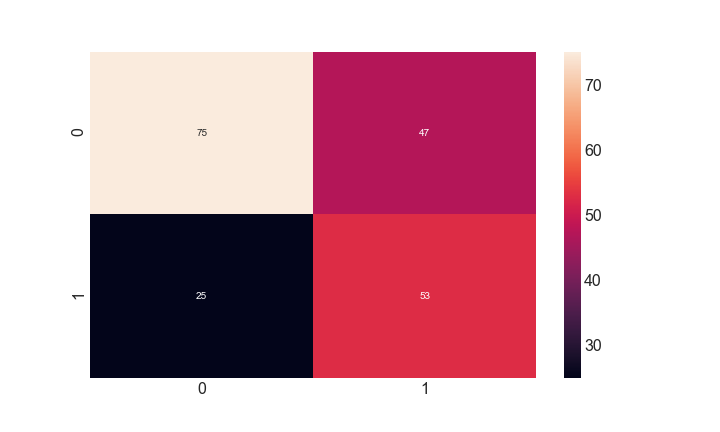
\includegraphics[width = \columnwidth]{grHOSgaus.png}
\caption{Link between clusters and labels (EM - initial BMW)}
\end{figure}

Hence, it appears that the two different clustering algorithms give us clusters totally different.

\section{Dimensionnality reduction algorithms}

We will now try to implement four dimension reduction algorithms on our two datasets. These algorithms are as follows: PCA, ICA, Random Projection, and SVD.

\subsection{PCA}

Let us recall the basic principle of the PCA. This algorithm tries to compose the initial space by projecting it onto orthogonal vectors, while maximizing the variance according to these vectors. Thus, if we note $X=\text{Span}\left(\{ x_i \} \right)$ the initial space, $X=\text{Span}\left(\{ y_j \} \right)$ the new projection space, we have the PCA algorithm which can be described as follows: 
\begin{itemize}
\item Initializing $l_y = \emptyset$ and $Y_0 = \text{Span}\left( l_y \right) $
\item Finding the vector $y_i$ in the orthogonal space of $Y_i$ that maximize the variance
\item Adding $y_i$ to $l_y$ and $Y_{i+1} =  \text{Span}\left( l_y \right)$
\item Repeating the two previous steps until $Y = X$ or we reach the limit number of vector we previously set.
\end{itemize}

\begin{figure}[H]
\centering
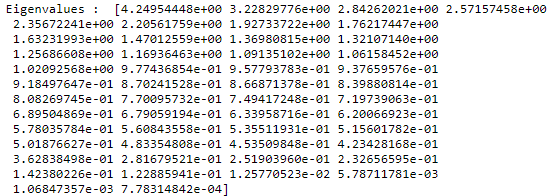
\includegraphics[width = \columnwidth]{eigenpcahos.png}
\caption{First Eigenvalues (PCA - HOS)}
\end{figure}

When using PCA, it is very interesting to look at the eigenvalues of the different vectors on which we project. Since we have previously normalized our data, an eigenvalue greater than 1 indicates that the axis in question represents more variance than one of the initial features. We can also look at their relative importance. For the representation in relation to certain axes, I have retained only a limited number of axes. However, for the reduction of dimensions I have retained the axes that give a variance greater than on the initial axes (which are 1).

\begin{figure}[H]
\centering
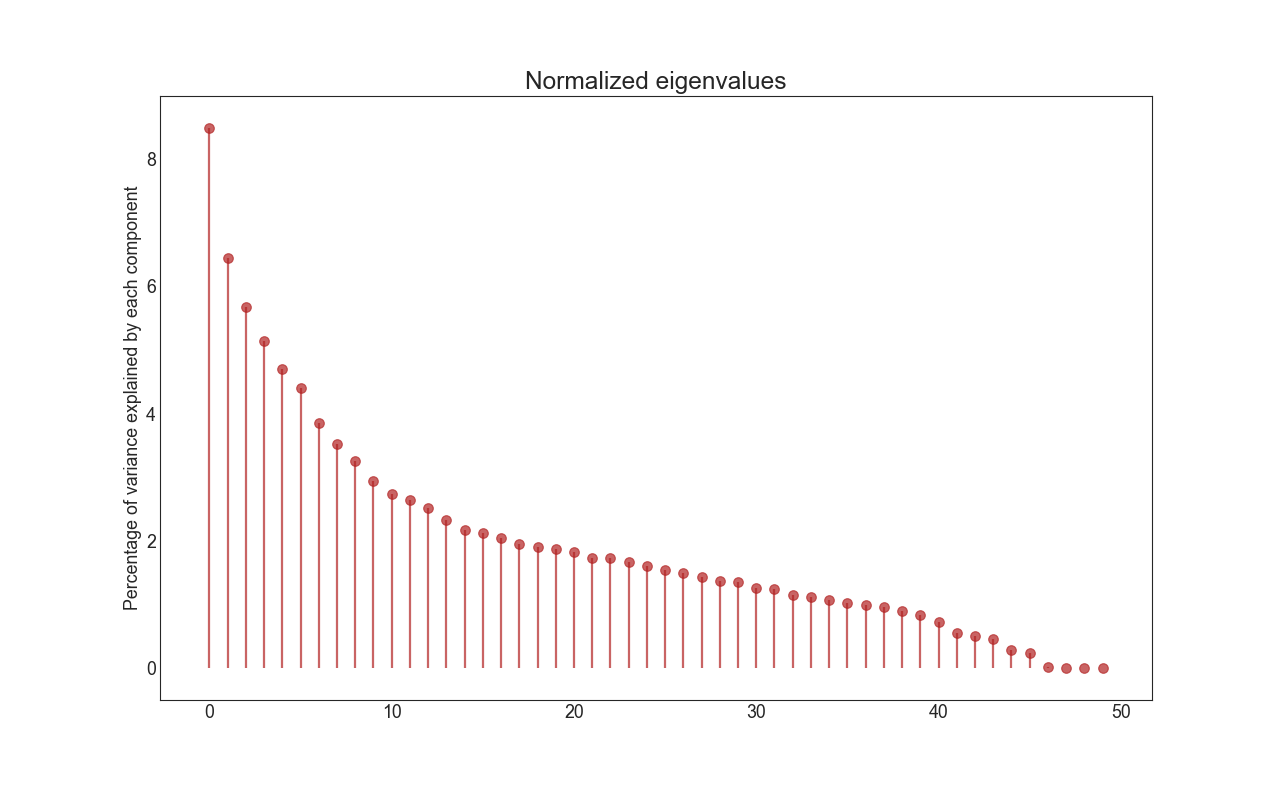
\includegraphics[width = \columnwidth]{egvHOSpca.png}
\caption{Relative importance of each Eigenvalues (PCA - HOS)}
\end{figure}

\begin{figure}[H]
\centering
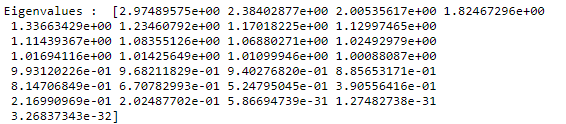
\includegraphics[width = \columnwidth]{eigenpcabmw.png}
\caption{First Eigenvalues (PCA - BMW)}
\end{figure}

\subsection{ICA}

In the context of the application of the ICA algorithm, we have already mentioned in the first part the conditions for the proper functioning of the algorithm (no Gaussian distribution, zero mean value...). But let's try to explain a bit more how it works. ICA tries to find vectors that are independent. For that, FastICA (which is one of the ICA implementation available on SKLearn) tries to maximize the non-gaussian measures. Indeed, given that the central limit theorem says that a sum of independent variables tends to a normal distribution, finding the components (vectors) that will maximize non-Gaussianity measures (such as the third or fourth order moment - Skew and Kurtosis) seems to be a good approach to determine variables that justify the group effect. Then, it then returns independent variables.

\subsection{Random projections}

The principle of the Random Projection algorithm is very simple and allows its execution at a particularly low time cost. It is simply to consider random linear combinations of the initial vectors and to take the projection of the data on the space defined by these new vectors. 

\subsection{SVD}

I have chosen to take as a fourth method the SVD. It does a similar job to PCA in the sense that it will define a new space according to the eigenvectors of the rectangular matrix associated to the set of our points. We can, afterwards, choose to truncate the decomposition we obtain to get the "best" approximation of the initial space in a restricted space. Also, in a similar way to the PCA algorithm, we can take a look at the distribution of the eigenvalues.

\begin{figure}[H]
\centering
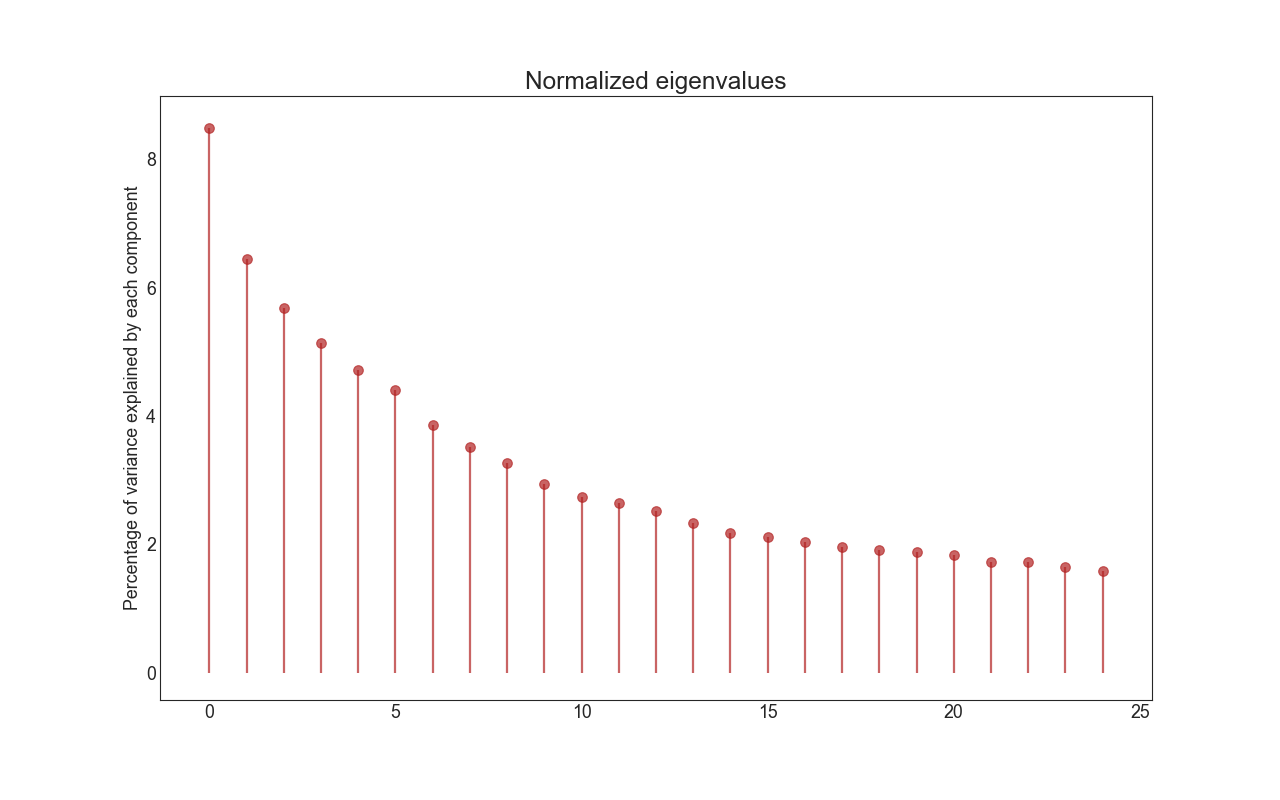
\includegraphics[width = \columnwidth]{egvHOSsvd.png}
\caption{Relative importance of each Eigenvalues (SVD - HOS)}
\end{figure}

\subsection{Reconstruction}

I have tried to evaluate the quality of reconstruction in the context of dimension reduction algorithms. To do this, for different values defining the number of dimensions on which we project our data, we perform the dimension reduction operation, then we use the inverse operator. We can summarize in this diagram:

$$X \underset{A}{ \rightarrow } P_X \underset{A'}{ \rightarrow } X' $$

I used the mean value of the Manhattan distance between $X$ and $X'$:

$$M = \frac{1}{n}\sum_{i=0}^{n-i} |x_i - x'_i|$$
to try to compare the different qualities of reconstruction according different algorithms. Surprisingly enough, I can't explain precisely why, the evolution of this measure is similar in most of the algorithms (PCA, ICA, SVD).

\begin{figure}[H]
\centering
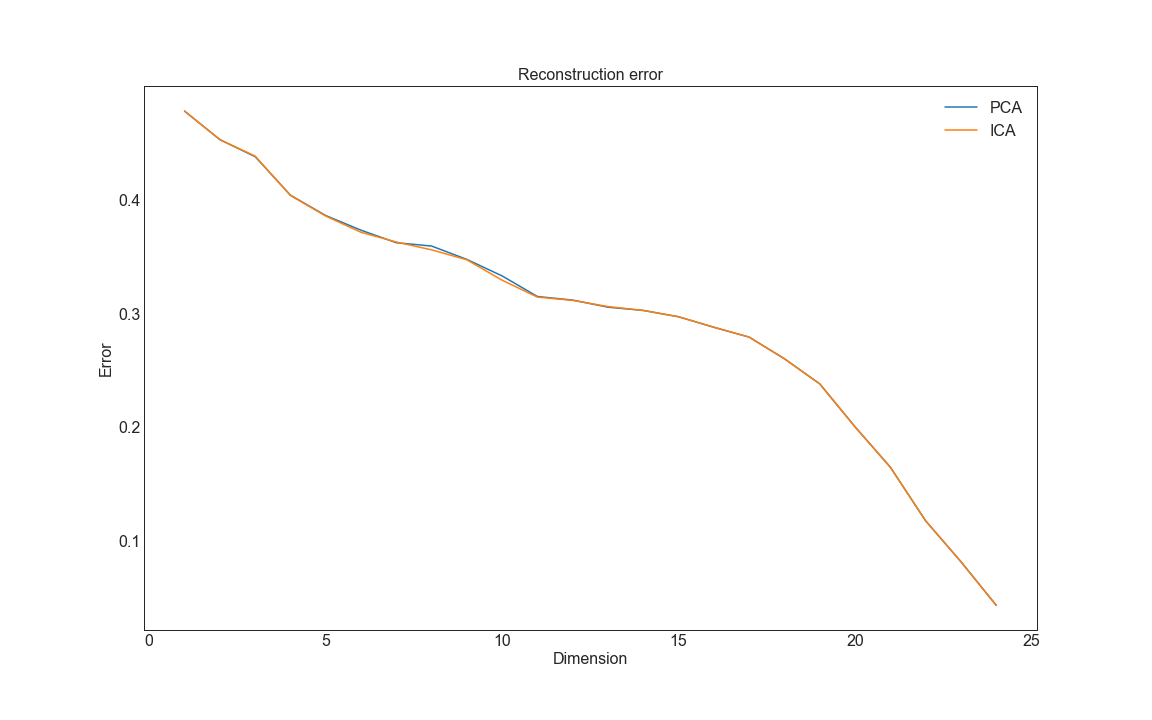
\includegraphics[width = \columnwidth]{errrecIPCA.png}
\caption{Mesure of the reconstruction error}
\end{figure}

In the framework of Random Projections, the reconstruction error depends not only on the number of dimensions on which we project our data but also on the random vectors chosen by the algorithm. To make a brief study of this method, for each dimension value, I have calculated the reconstruction error on a hundred Random Projections and I have displayed the average value of the reconstruction error and its range of variation.

\begin{figure}[H]
\centering
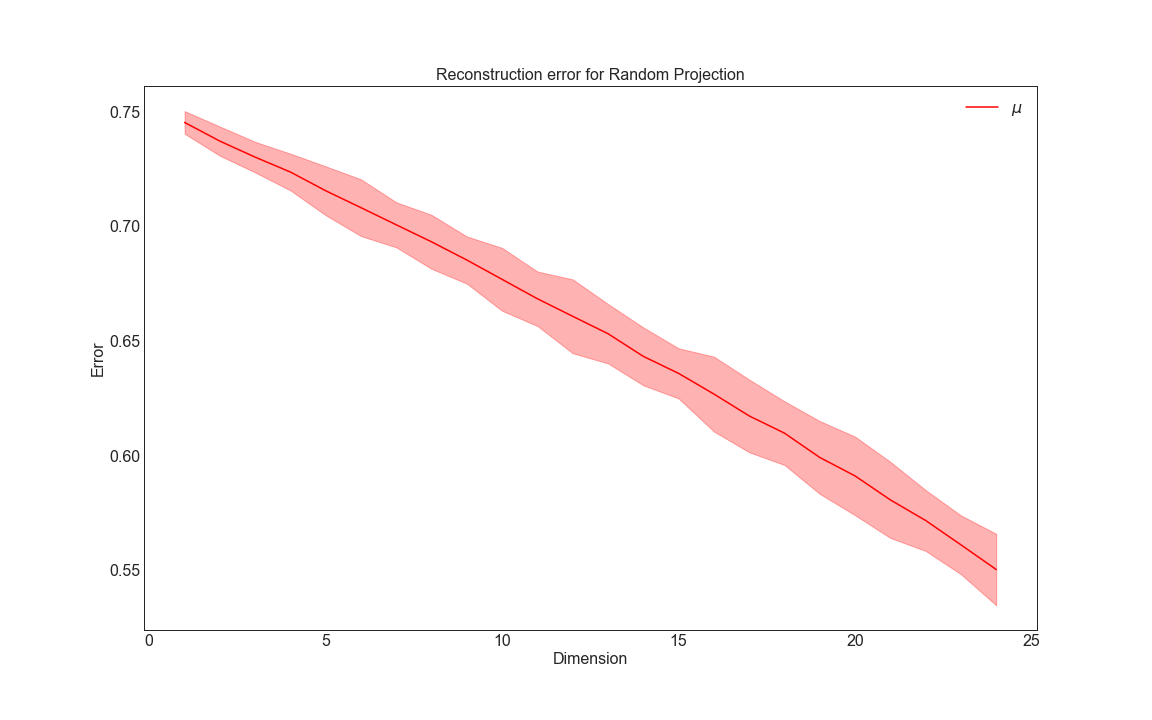
\includegraphics[width = \columnwidth]{HerrrecRandom.png}
\caption{Reconstruction error with Random Projections}
\end{figure}

\section{Clustering on reduced datasets}

We now want to combine the use of clustering algorithms with those of dimension reduction to study the possibility of recovering new insights on our initial datasets. Moreover, it is interesting to see if the clusters we obtain are similar to the previous ones.

On each dataset passed by a dimension reduction algorithm, I tried again to perform the elbow method and in most cases a slight break appeared and allowed me to determine a value for the hyperparameter.

\begin{figure}[H]
\centering
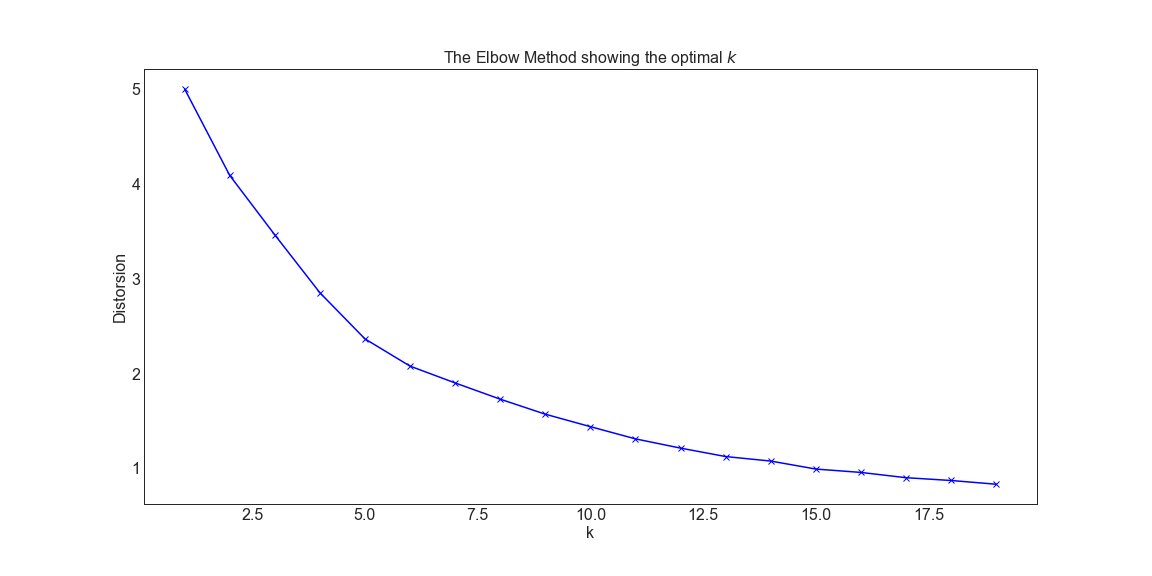
\includegraphics[width = \columnwidth]{elbowkmpca.png}
\caption{Elbow method (KM - PCA BMW)}
\end{figure}

However, in most cases, and mainly in the case of the medical dataset, I performed a clustering with a different hyperparameter than the one used during the exploration of the initial datasets. Thus, in a natural way, the clusters that we will have defined after the use of the dimension reduction algorithms are different from the first ones.

\begin{figure}[H]
\centering
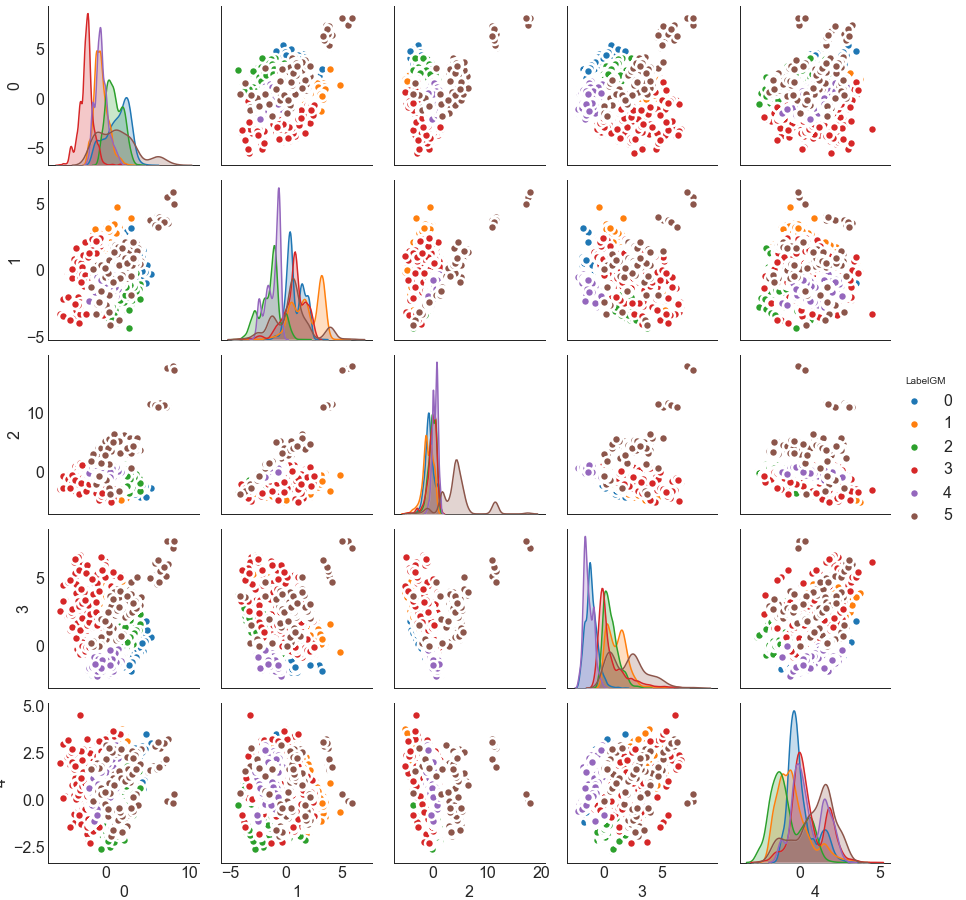
\includegraphics[width = \columnwidth]{pplotBMWgmpca.png}
\caption{Cluster projections over principal features (GM - PCA BMW)}
\end{figure}

We can still try to compare the clusters that come from this step with the labels that were originally associated with our data to try to discern the ability of the clustering algorithms to structure the data in a way that is relevant for the future prediction of labels.

If we reconsider the use of the EM method on the BMW dataset (which is now processed by PCA), we can see that the clusters constructed make more sense than the use of EM alone.



\begin{figure}[H]
\centering 
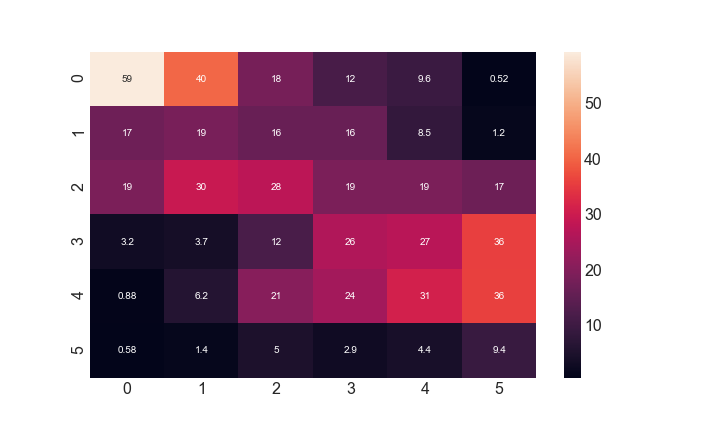
\includegraphics[width = \columnwidth]{grBMWgmpca.png}
\caption{Link between clusters and labels (EM - PCA BMW)}
\end{figure}

\begin{figure}[H]
\centering
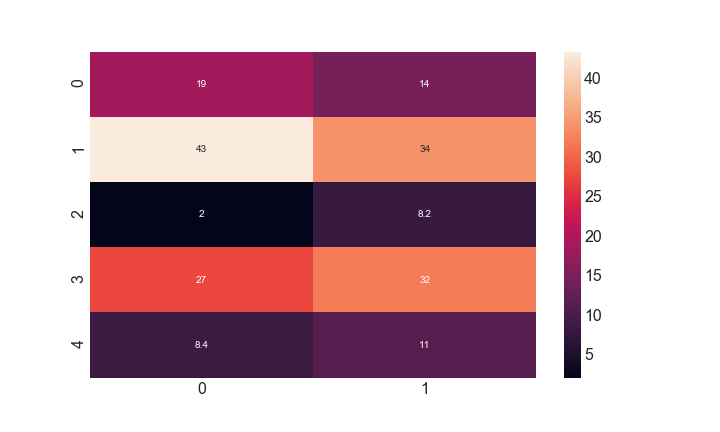
\includegraphics[width = \columnwidth]{grhosgmica.png}
\caption{Clustering not really useful (EM-ICA HOS)}
\end{figure}

We can thus observe that contrary to the first clustering using EM which had gathered the majority of the datapoints under the same cluster. Here, we can perceive that some cluters will define correct indicators to later try to find the labels of the datasets. Here, it looks like the Gaussian random variables that EM defined covers a label and its nearest neighbors. I mean: cluster 0 covers mainly the cheapest vehicles (label 0 and 1) and a bit of the mid-range, cluster 1 would tend to cover the vehicles halfway between the low and mid-range, cluster 2 covers the mid-range... Here the clustering conceals a structure that sheds light on the dataset.

When we observe the results of clustering on other datasets, the results are very different. In some cases, to my eyes, we don't really seem to obtain a coherent structure (in the sense of "making sense") of our dataset, while for others a slight understanding of the dataset seems to appear.



\begin{figure}[H]
\centering
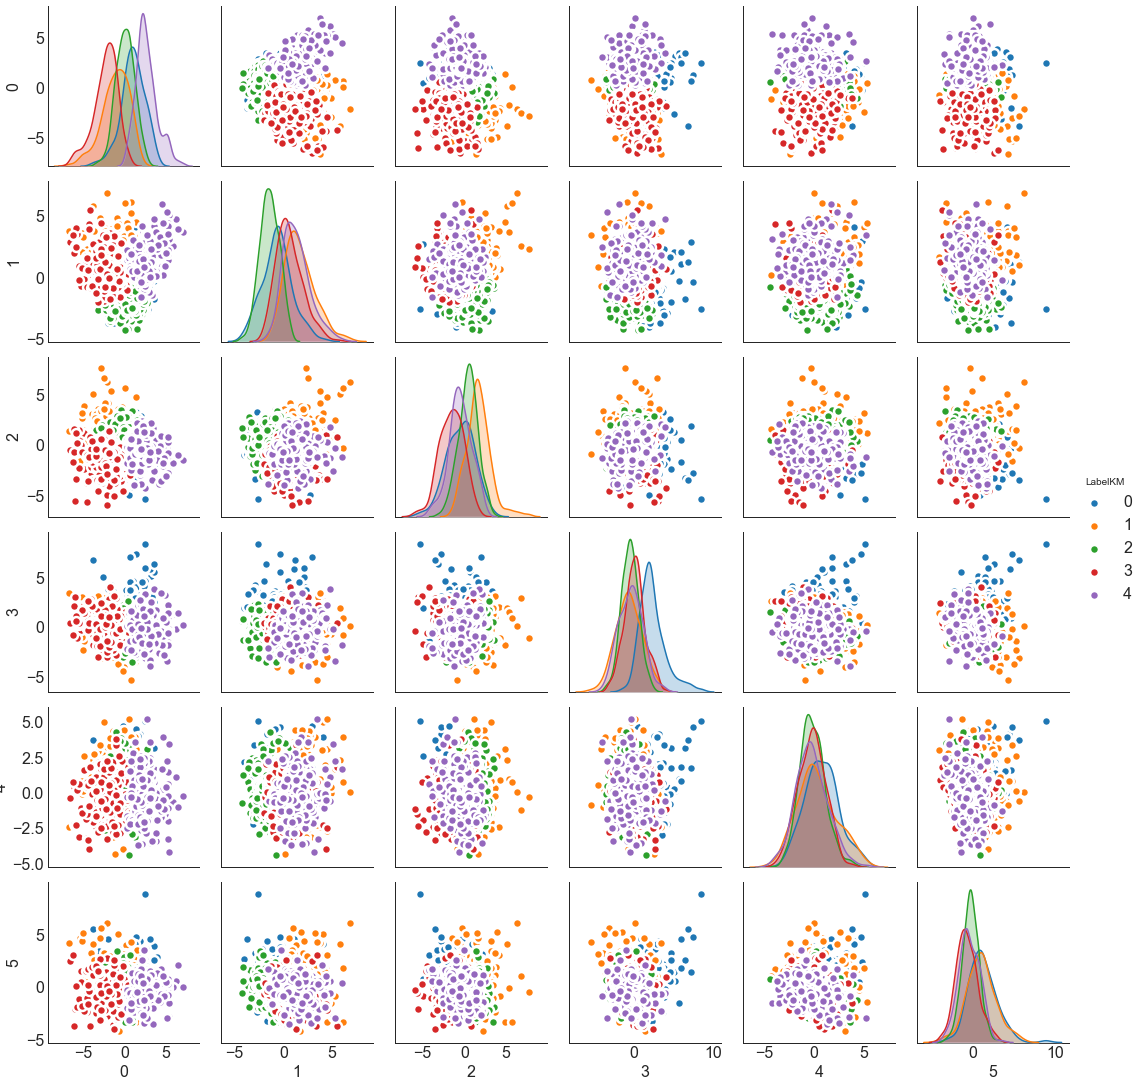
\includegraphics[width = \columnwidth]{pplothoskmsvd.png}
\caption{Projections (KM - SVD HOS)}
\end{figure}

\begin{figure}[H]
\centering
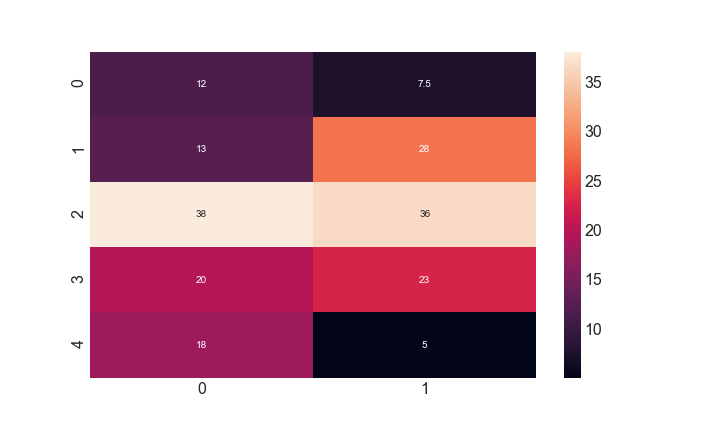
\includegraphics[width = \columnwidth]{grhoskmsvd.png}
\caption{Clustering useful? (KM-SVD HOS)}
\end{figure}

\section{Construction of models: Neural Networks}

It is now time to look at the use of these algorithms in the context that interests us most: Machine Learning. Clustering and dimension reduction algorithms are indeed tools that can help us to improve the datasets on which we will build our models. We want to see if we can perceive the influence of these algorithms on the performance of a model. That's why we will discuss the construction of a Neural Network. I choose to run a Neural Network on the mortality dataset. Below we can find the learning curve corresponding for some datasets (initial or transformed). The precision metric is the accuracy score and we use a 5-folds cross-validation when we mesure cross-validation score.

\begin{figure}[H]
\centering
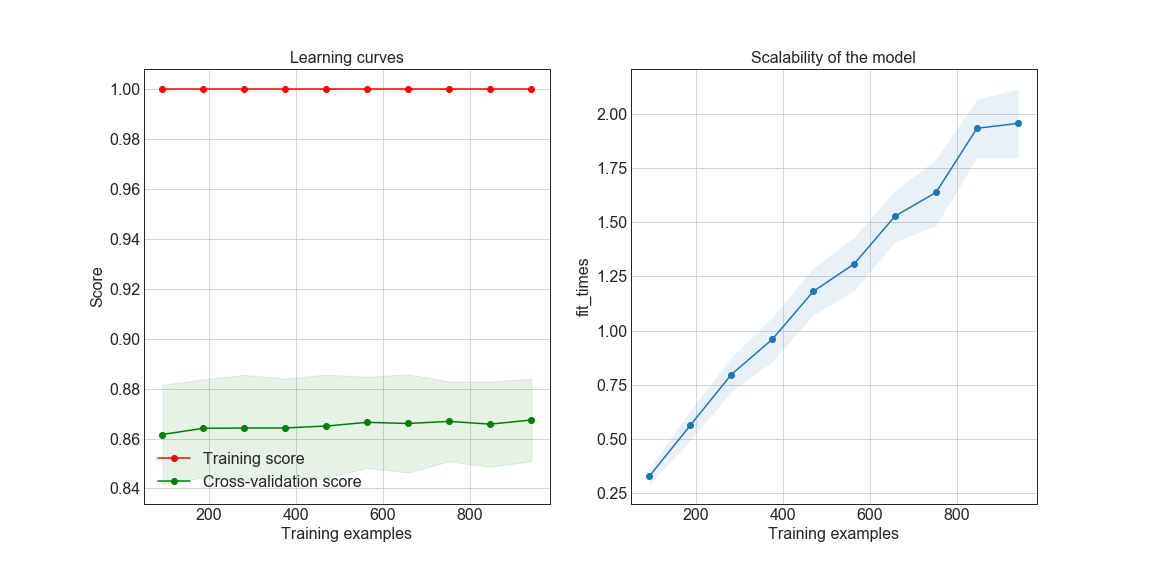
\includegraphics[width = \columnwidth]{NNC2.png}
\caption{Neural Network learning curves on initial dataset}
\end{figure}

\begin{figure}[H]
\centering
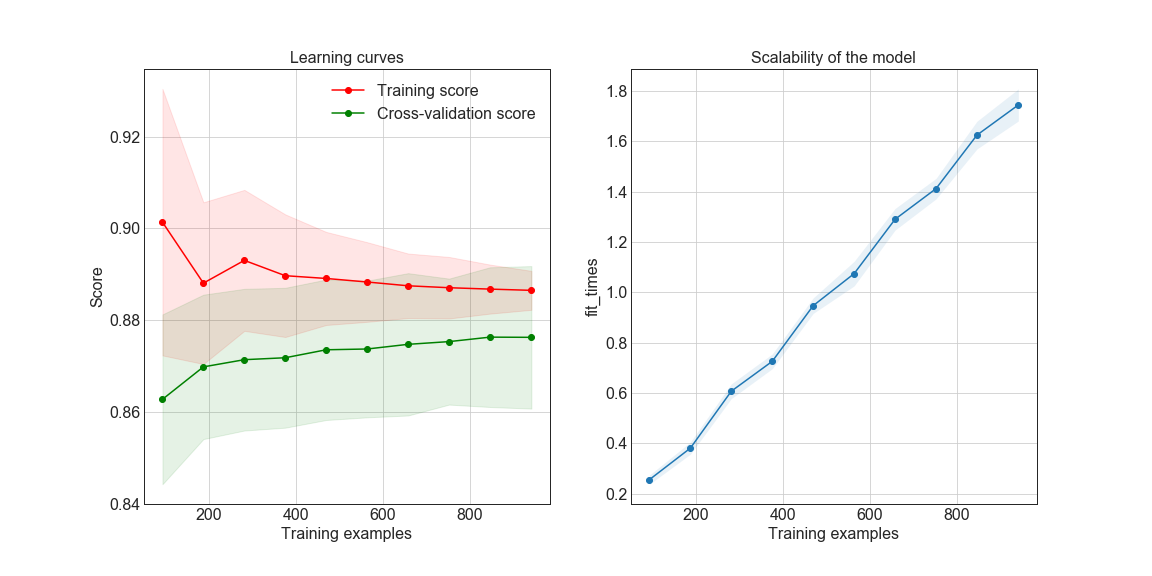
\includegraphics[width = \columnwidth]{NNCpca.png}
\caption{Neural Network learning curves on PCA dataset}
\end{figure}

\begin{figure}[H]
\centering
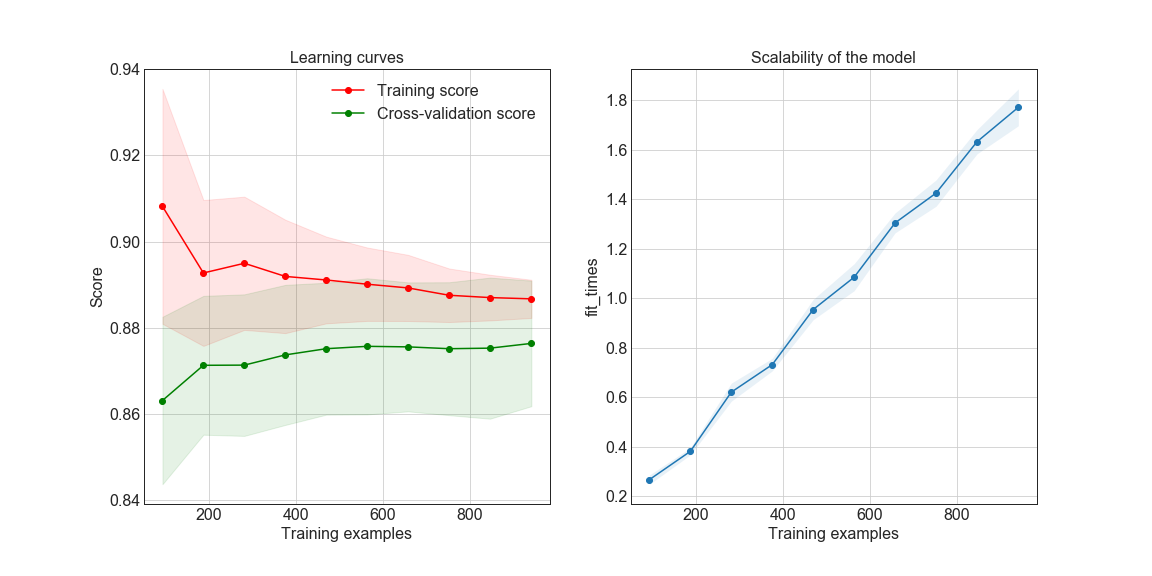
\includegraphics[width = \columnwidth]{NNCkmpca.png}
\caption{Neural Network learning curves on KM-PCA dataset}
\end{figure}

\begin{figure}[H]
\centering
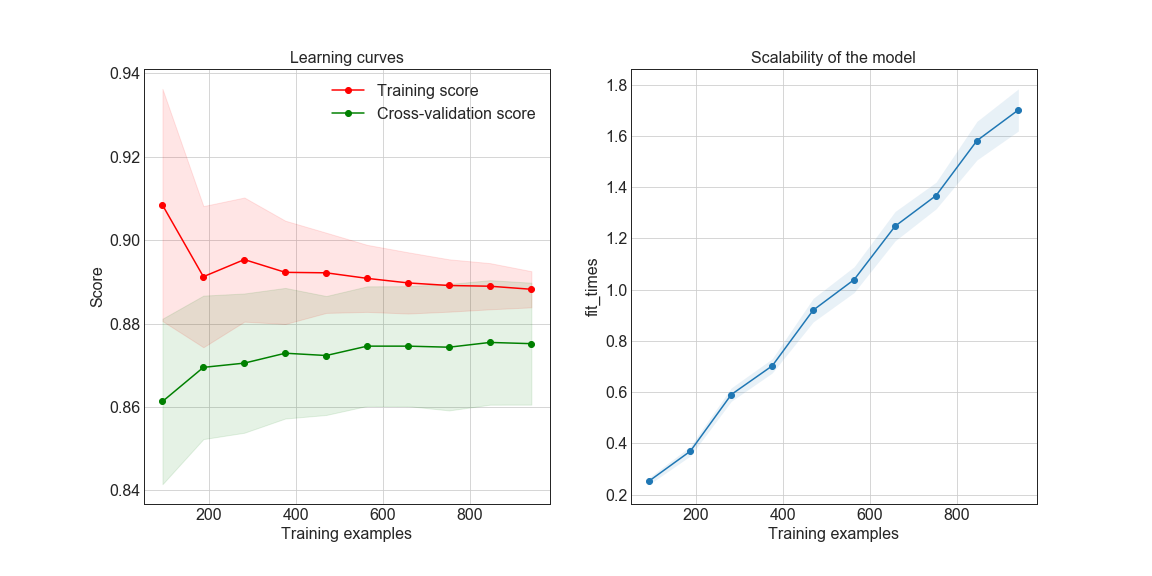
\includegraphics[width = \columnwidth]{NNCgmpca.png}
\caption{Neural Network learning curves on EM-PCA dataset}
\end{figure}

The first graph will be used as a reference since it corresponds to the construction of a Neural Network on the initial dataset (on which we have just operated a StandardScaler). The second one corresponds to the case where we use the dataset on which we have applied a PCA, the third one where we have applied a PCA and added in feature the labels of a KMeans, while the last one is the one where we have applied a PCA and added in feature the EM labels. 

This choice to focus on the latter is in the will to focus on performance changes due to the use of clustering and dimension reduction algorithms and not caused by the application of different dimension reduction algorithms.

If we focus on predictive capabilities:
\begin{itemize}
\item Comparing the first two graphs, we can see that the reduction in dimension has not particularly degraded the predictive capacity (cross validation score) of the model.
\item Comparing the last two to the previous ones, we can see a slight improvement of the scores with the use of clusters as new features
\item The overfitting is less in the case of models using reduced dimension datasets (but this is mainly due to the collapse of the score on the training sets).
\end{itemize}
Now if we look at the temporal aspect of the model construction, this is where we find a real difference. Indeed, the dimension reduction allows to simplify, to purify the model. This allows us to run a faster optimization of the Neural Network coefficients. We note here an improvement of a little more than ten percent in terms of time. 

\section{Conclusion}

Clustering algorithms seem to be very appropriate to find a structure within a dataset. Indeed, this is the main goal of these algorithms: to group within clusters points being similar (modulo the definition of similarity). But it also appears that the use of these algorithms is interesting in the context of Supervised Learning problems. Indeed, they can contribute to the construction of new features allowing to retranscribe this similarity that models (considering the features in a more individual way) could perhaps not perceive.

Dimension reduction algorithms are also important, even indispensable in the context of real life applications. Indeed, the real applications of Machine Learning have more and more tendency to focus on very large datasets favored by the current tendency to accumulate all available information. Already, on our small scale, we could perceive the effects of these algorithms which allow, with a reasonable degradation of the dataset information, to have models with similar predictive performances but with a much more efficient implementation at the temporal level.

\end{multicols}

\end{document}